\section{Design of the Delay and \gls{reverb} Effect}
In this section, the delay and the \gls{reverb} will be designed to fit intro a \gls{dsp}, which mean that a discreet block diagram is obtained and afterwords the equation to the implementation is made. All the equation will afterwords be simulated in MATLAB and then the assembly code is developed and implemented. 


\subsection{Obtaining the Differential Equation}
The Delay and \gls{reverb} effect are very similar in their design so they will be presented and designed in the same section. The block diagram presented in \autoref{} is changed so it fit intro a direct form 2 construction. This effect both have \gls{iir} filter and \gls{fir} filter, but it is only the \gls{iir} filter which make the echo, the \gls{fir} filter is only applied to make a flat frequency respond. To get a naturally \gls{reverb} effect with the identical respond as a room acustic respond and avoiding fluttering, all the seriel \gls{reverb} unit needs to be an all pass filter and all parallel \gls{reverb} unit needs to be low pass filter. The low pass filter is used because the room akustic caristica is acting as a low pass filter, all low frequency signal will stay longer in the room than the high frequency \autoref{}.  The \gls{reverb} needs to have at least 1000 echo per second, and the best way to make the \gls{reverb} effect is with four low pass \gls{iir} filters and 2 all pass filter otherwise if all the all pass filter was in parallel, it will require forty all pass filter to make 1000 echo per second \citep{natural_sounding_revorb}. The block diagram \autoref{fig:reverb_block_des} is in direct form 2 to minimize the implementation program. The delay and \gls{reverb} effect can be obtained and is shown in \autoref{fig:reverb_block_des}. The \gls{reverb} effect is the one in red and black while the delay is only in red. 

\newpage

\begin{figure} [htbp]
 \centering
\begin{picture}(0,0)%
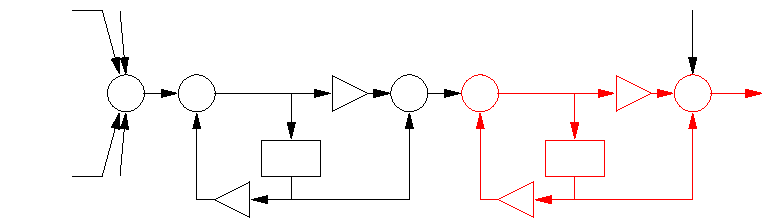
\includegraphics{reverb_diag_des.pdf}%
\end{picture}%
\setlength{\unitlength}{4144sp}%
%
\begingroup\makeatletter\ifx\SetFigFont\undefined%
\gdef\SetFigFont#1#2#3#4#5{%
  \reset@font\fontsize{#1}{#2pt}%
  \fontfamily{#3}\fontseries{#4}\fontshape{#5}%
  \selectfont}%
\fi\endgroup%
\begin{picture}(5832,1599)(-1319,-1288)
\put(2656,-106){\color[rgb]{1,0,0}$w_6[n]$}%
\put(1711,-421){$\Sigma$}%
\put(721,-916){$z^{-d_5}$}%
\put( 91,-421){$\Sigma$}%
\put(1261,-196){$-a_5$}%
\put(2251,-421){\color[rgb]{1,0,0}$\Sigma$}%
\put(2881,-916){\color[rgb]{1,0,0}$z^{-d_6}$}%
\put(271,-1006){$a_5$}%
\put(2431,-1006){\color[rgb]{1,0,0}$a_6$}%
\put(3871,-421){\color[rgb]{1,0,0}$\Sigma$}%
\put(3421,-196){\color[rgb]{1,0,0}$-a_6$}%
\put(-449,-421){$\Sigma$}%
\put(-224,-106){$x_5[n]$}%
\put(1936,-106){\color[rgb]{1,0,0}$x_6[n]$}%
\put(4276,-106){\color[rgb]{1,0,0}$y[n]$}%
\put(-1304,-151){Low pass}%
\put(-1304,-421){filter in}%
\put(-1304,-646){Parallel}%
\end{picture}%

  \caption{The figure shows a block diagram of a \gls{reverb} and delay unit.}
  \label{fig:reverb_block_des}
\end{figure}

From \autoref{fig:reverb_block_des}, the following differential equations can be inferred for the delay, where the number 6 is omitted since the delay effect only is the the red.

\begin{subequations}
\begin{equation}\label{eq:delay_eq}
       y[n] = - \alpha \cdot w[n] + w[n-d]
    \end{equation}
\begin{equation}\label{eq:delay_eq_in}
       w[n] = \alpha \cdot w[n-d] + x[n] 
    \end{equation}
 \end{subequations}
		
		

The \gls{reverb} unit is more advanced than the delay unit and before the differential equations can be inferred, some calculation is needed. The \gls{reverb} unit calculation are based on a article \citep{natural_sounding_revorb} which explain the design parametric for a \gls{reverb} unit very well. Form \citep{natural_sounding_revorb} the \gls{reverb} time is defined by \autoref{eq:reverb_defined}



\begin{equation}
\label{eq:reverb_defined}
		T = \frac{60}{-20 \cdot log(\alpha)} \cdot \tau
\end{equation}

    \startexplain
\explain{$60$ is the \gls{reverb} attenuation in \si{\decibel}, and the \gls{reverb} time is defined that a given signal is attenuated by 60 \si{\decibel}}{\si{\decibel}}
\explain{$\tau$ is the delay time}{\si{\second}}
\explain{$T$ is the resulting \gls{reverb} time}{\si{\second}}
\explain{$-20 \cdot log10(\alpha)$ is the attenuation in the feedback loop for each round}{\si{\decibel}}
    \stopexplain

Both the positive and negative gain $\alpha$ is defined to be 0.75  \citep{natural_sounding_revorb} and the total \gls{reverb} echo density shall at lest be 1000 echo per second. In formula \autoref{eq:reverb_defined_tal_res} it can be obtain that $\tau$ shall be $\frac{1}{24}$ of $T$


\begin{subequations}
\begin{equation}\label{eq:reverb_defined_tal}
       T = \frac{60}{-20 \cdot log10(0.75)} \cdot \tau
       \addunit{\si{\second}}
    \end{equation}
\centering
$\Updownarrow$
\begin{equation}\label{eq:reverb_defined_tal_res}
        \tau = \frac{1}{24} T
        \addunit{\si{\second}}
    \end{equation}
 \end{subequations}

\autoref{eq:reverb_defined_tal_res} then shows that the $\tau$ time is \SI{42}{\milli\second} with a total \gls{reverb} time $T$ of \SI{1}{second}. This achieve an echo density of 24 echo per second for each of the \gls{iir} low pass filter, but if all the filter have the same delay time some echo will interference. To avoid interference each filter delay time is chosen to its own prime numbers which lay nearest \SI{42}{\milli\second}. The chosen delay prime number is as following \autoref{tab:reverb_delay}

\begin{table}[htbp]
\centering
\caption{The chosen delay prime numbers}
\label{tab:reverb_delay}
\begin{tabular}{lll}
$d_1$ & = & 37 \\
$d_2$ & = & 41 \\
$d_3$ & = & 43 \\
$d_4$ & = & 47 \\
$d_5$ & = & 29 \\
$d_6$ & = & 31
\end{tabular}
\end{table}

Each \gls{iir} filter is also attenuated by a defined gain which is shown in \autoref{tab:reverb_bgain}

\begin{table}[htbp]
\centering
\caption{The chosen delay prime numbers}
\label{tab:reverb_bgain}
\begin{tabular}{lll}
$b_1$ & = & 1 \\
$b_2$ & = & 0.9 \\
$b_3$ & = & 0.8 \\
$b_4$ & = & 0.7 
\end{tabular}
\end{table}


The \gls{reverb} unit require 1000 echo per second \citep{natural_sounding_revorb}. To achieve 1000 echo per second there needs to be multiply all pass \gls{fir} filter delay unit in serial after the four in parallel defined \gls{iir} low pass filter. It is defined by \citep{natural_sounding_revorb} that two \gls{fir} filter is required. To calculate the approximated number of echo in one second from the 4 \gls{iir} filter, the following \autoref{eq:reverb_par} calculation the echo, where the two first \gls{iir} filters is 24 echo since the prime number is under 42.

\begin{subequations}
\begin{equation}\label{eq:reverb_par}
       \text{Numbers of echo in \gls{iir} filter} = 24 + 24 + \left \lfloor \frac{1000}{43}  \right \rfloor + \left \lfloor \frac{1000}{47}  \right \rfloor
       \addunit{\si{1}}
    \end{equation}
\centering
$\Updownarrow$
\begin{equation}\label{eq:reverb_parres}
        \text{Numbers of echo in \gls{iir} filter} = 92
        \addunit{\si{1}}
    \end{equation}
 \end{subequations}

The following calculation \autoref{eq:reverb_ser} calculate the approximate resulting echo after the first \gls{fir} filter. Both the first and the second \gls{fir} have a prime number under 42, so each signal from the \gls{fir} filter will be repeated maximum of $24-1$ times before the signal is attenuated under \SI{60}{\decibel}.


\begin{subequations}
\begin{equation}\label{eq:reverb_ser}
      \text{aprox numbers of echo from first \gls{fir} filter} = \sum_{x=1}^{23} 24-x + \sum_{x=1}^{20} 24-x + \sum_{x=1}^{18} 23-x + \sum_{x=1}^{14} 21-x
       \addunit{\si{1}}
    \end{equation}
\centering
$\Updownarrow$
\begin{equation}\label{eq:reverb_seriel}
        \text{aprox numbers of echo from first \gls{fir} filter} = 942
        \addunit{\si{1}}
    \end{equation}
 \end{subequations}

    \startexplain
\explain{$20$ is calculated from each echo from the second \gls{iir} filter which is attenuated 10 percent, $echo=\left \lfloor 24-1 \cdot b_2 \right \rfloor$ }{\si{1}}
\explain{$18$ is calculated from each echo from the third \gls{iir} filter which is attenuated 20 percent, $echo=\left \lfloor 23-1 \cdot b_3 \right \rfloor$ }{\si{1}}
\explain{$14$ is calculated from each echo from the fourth \gls{iir} filter which is attenuated 30 percent, $echo=\left \lfloor 21-1 \cdot b_4 \right \rfloor$ }{\si{1}}
    \stopexplain

Since the echo density already is about 942 echo per second, the last \gls{fir} filter will ensure over 1000 echo per second from the output of the \gls{reverb} effect. The following \autoref{fig:reverb_block_design} shows a direct form 2 block diagram over the \gls{reverb} unit.

\begin{figure} [htbp]
 \centering
\begin{picture}(0,0)%
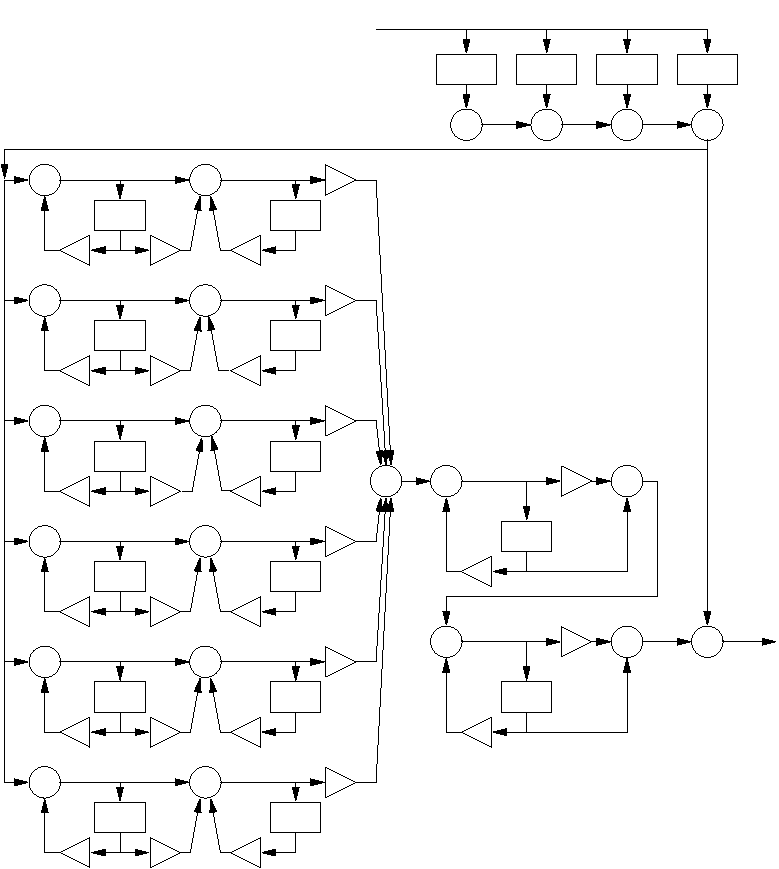
\includegraphics{reverb_serial_des.pdf}%
\end{picture}%
\setlength{\unitlength}{3274sp}%
%
\begingroup\makeatletter\ifx\SetFigFont\undefined%
\gdef\SetFigFont#1#2#3#4#5{%
  \reset@font\fontsize{#1}{#2pt}%
  \fontfamily{#3}\fontseries{#4}\fontshape{#5}%
  \selectfont}%
\fi\endgroup%
\begin{picture}(7317,5055)(-2804,-3178)
\put(-944,434){$b_2$}%
\put(1711,-421){$\Sigma$}%
\put(721,-916){$z^{-d_5}$}%
\put( 91,-421){$\Sigma$}%
\put(1261,-196){-$\alpha_5$}%
\put(2251,-421){$\Sigma$}%
\put(2881,-916){$z^{-d_6}$}%
\put(271,-1006){$\alpha_5$}%
\put(2431,-1006){$\alpha_6$}%
\put(3871,-421){$\Sigma$}%
\put(3421,-196){$-\alpha_6$}%
\put(-449,-421){$\Sigma$}%
\put(-2024,-421){$\alpha_2$}%
\put(-2159,209){$\Sigma$}%
\put(-1529,-286){$z^{-d_2}$}%
\put(-1529,-1546){$z^{-d_3}$}%
\put(-2789,-286){$x[n]$}%
\put(-1529,-2806){$z^{-d_4}$}%
\put(-2159,-2311){$\Sigma$}%
\put(-2024,-2941){$\alpha_4$}%
\put(-944,-2086){$b_4$}%
\put(-2024,-1681){$\alpha_3$}%
\put(-1529,974){$z^{-d_1}$}%
\put(-944,1694){$b_1$}%
\put(-2159,1469){$\Sigma$}%
\put(-2024,839){$a_1$}%
\put(1936,-196){$x_6[n]$}%
\put(4276,-196){$y[n]$}%
\put(-224,-196){$x_5[n]$}%
\put(-1619,1649){$x_1[n]$}%
\put(-1619,389){$x_2[n]$}%
\put(-1619,-871){$x_3[n]$}%
\put(-1619,-2131){$x_4[n]$}%
\put(-2159,-1051){$\Sigma$}%
\put(-944,-826){$b_3$}%
\end{picture}%
  \caption{The figure shows a block diagram of a \gls{reverb} unit.}
  \label{fig:reverb_block_design}
\end{figure}


The equation for the \gls{reverb} can be written in six parts as:


\begin{subequations}
\begin{equation}\label{eq:reverb_eq_1}
x_5[n] = ((x[n]+x_1[n-d_1] \cdot \alpha_1) \cdot b_1)+((x[n]+x_2[n-d_2] \cdot \alpha_2) \cdot b_2)+((x[n]+x_3[n-d_3] \cdot \alpha_3) \cdot b_3)+((x[n]+x_4[n-d_4] \cdot \alpha_4) \cdot b_4)
    \end{equation}
\begin{equation}\label{eq:reverb_eq_2}
x_6[n] = - \alpha_5 \cdot w_5[n] + w_5[n-d_5]
    \end{equation}
\begin{equation}\label{eq:reverb_eq_3}
w_5[n] = \alpha_5 \cdot w[n-d_5] + x_5[n] 
    \end{equation}
    \begin{equation}\label{eq:reverb_eq_4}
y[n] = - \alpha_6 \cdot w_6[n] + w_6[n-d_6]
    \end{equation}
    \begin{equation}\label{eq:reverb_eq_5}
w_6[n] = \alpha_6 \cdot w[n-d_6] + x_6[n] 
    \end{equation}
 \end{subequations}


\subsection{Matlab Simulation}

A delay can be done in different ways digitally. One way is to use a ring buffer also known as circular buffer. \\
The idea of this data structure is that it takes values and only outputs them when it gets full, and overwrites the oldest after outputting it. It is a kind of a FIFO queue structure but where the start and the overwriting can start at any index. \\
This means that the size of the buffer depends on the delay.  The buffer size must then be always up-to-date with the new delay value. \\ 

The Matlab code for the delay effect is as following \autoref{code:delay_sim}

\includeCode{delay.m}{matlab}{1}{39}{The delay simulation matlab code}{code:close}{code/design/}\label{code:delay_sim}


Applying one sinus round gives the following result

\begin{figure}[htbp]
	\centering
	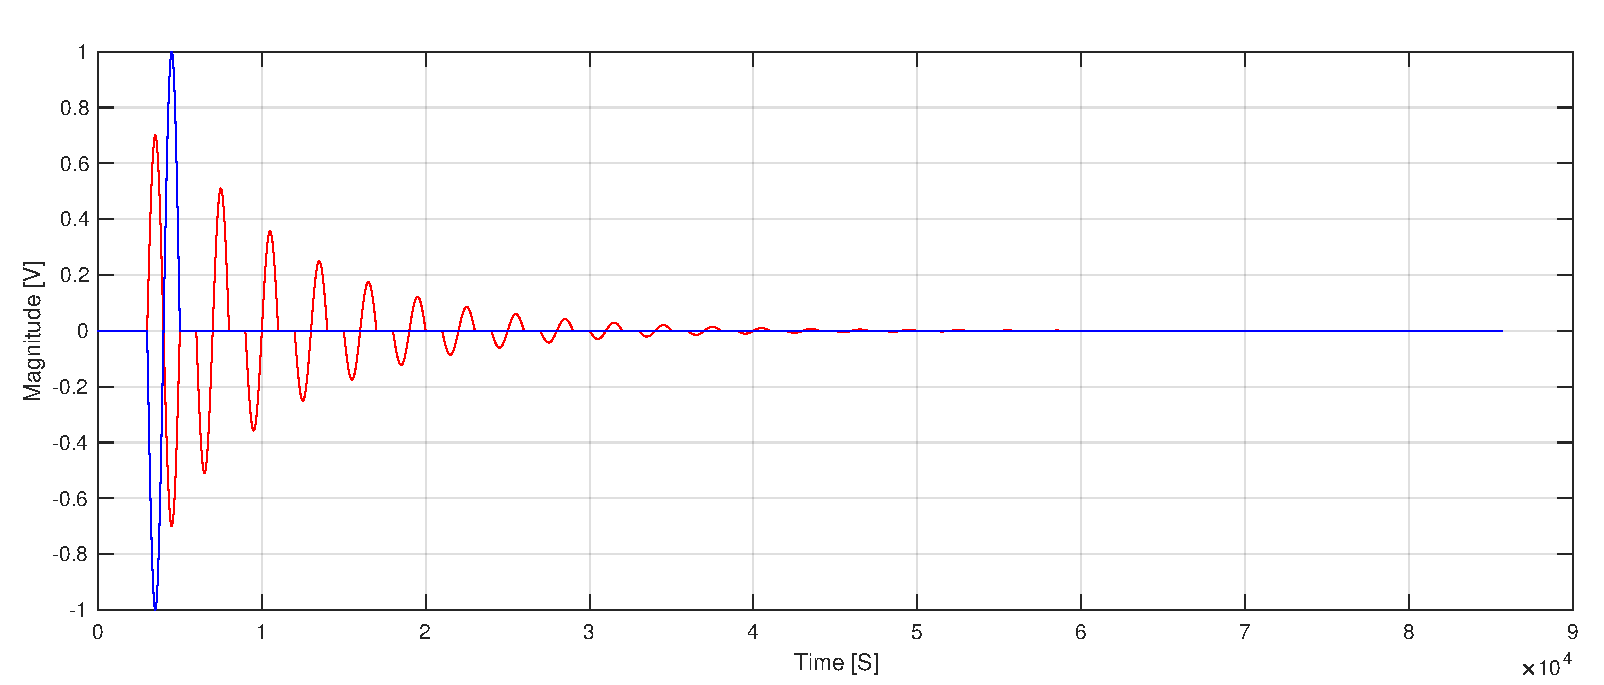
\includegraphics[width=1\textwidth]{delay}
	\caption{The plot shows the result for the \autoref{code:delay}}
	\label{fig:delay_plot}
\end{figure}